\documentclass{article}
\usepackage{graphicx} % Required for inserting images


\title{GLM Assignment 1}
\author{Parth Gupte}
\date{March 2024}

\begin{document}

\maketitle

\section{Introduction}
In the given problem we are asked to model the proportion of people who 
pass the test using data about which treatments they were given and in what doses.
There are 2 types of treatments being delivered to the patients, Treat1 and Treat2.
In each treatment they are given one of two medicines, for Treat1,
they are given medicines A or B and for Treat2 they are given medicines X or Y.\\
We are also given the amount of dose of each treatment given to 
the subjects Dose1 and Dose2.\\

\section{Models Tried}
I tried 4 basic types of models and repeated these for all the 3 binomial
link functions. These are as listed below:\\
\\
\subsection{Simple Sum}
In this model I simply performed GLM regression on 
Pass/Total against the 4 columns of the data in a sum.\\
\\
This model can be represented by the following R formula:\\
\begin{verbatim}
    Pass/Total ~ Treat1 + Dose1 + Treat2 + Dose2    
\end{verbatim}

\subsection{Product of Treatment and Dose}
In this model I regressed Pass/Total against:\\
Treat1AxDose1, Treat1BxDose1, Treat2XxDose2, Treat2YxDose2.\\
Where Treat1A is 1 when medicine A is given in treatment 1 and similarly for others.
The reasoning behind this is that the amount of dose can have different
amount of effect based of if medicine A was given or B.
In all the cases this reduces the residual Deviance.\\
\\
This model is represented by the following R formula:\\
\begin{verbatim}
    Pass/Total ~ Treat1:Dose1 + Treat2:Dose2
\end{verbatim}

\subsection{Cross Terms}
In this model I added all the cross terms of Treatment and Dose.\\
Pass/Total was regressed against the products of doses and treaments as in the 
previous model but the simple terms of Treat1, Treat2, Dose1 and Dose2 were also added.
This model gives a further improvement in performance in all the link functions.\\
\\
This model is represented by the following R formula:\\
\begin{verbatim}
    Pass/Total ~ Treat1*Dose1 + Treat2*Dose2
\end{verbatim}

\subsection{Partial Cross Terms}
In the analysis of the previous model I observed that out
of the linear terms only the coefficients for treatment terms were significant
hence for finding a maximum parcimonious model I kept only those terms.
This model has the same performance as the previous model but has lesser parameters.
This can be interpreted as perhaps the effect increases linearly with dose but with non zero intercept.\\
\\
This model is represented by the following R formula:\\
\begin{verbatim}
    Pass/Total ~ Treat1:Dose1 + Treat2:Dose2 + Treat1 + Treat2
\end{verbatim}

\section{Results}
These models were evaulated for all 3 link functions, logit, probit and loglog.
Out of these loglog gave the best performance with model 4.\\
\\
The metrics of the fit are as follows:\\
\begin{verbatim}
    glm(formula = Pass/Total ~ Treat1:Dose1 + Treat2:Dose2 + Treat1 + 
    Treat2, family = binomial(link = "cloglog"), data = data, 
    weights = Total)

    Coefficients:
                   Estimate Std. Error z value Pr(>|z|)    
    (Intercept)    0.572205   0.201273   2.843  0.00447 ** 
    Treat1B       -0.385280   0.135149  -2.851  0.00436 ** 
    Treat2Y       -0.833672   0.276225  -3.018  0.00254 ** 
    Treat1A:Dose1 -0.019452   0.013488  -1.442  0.14926    
    Treat1B:Dose1  0.066677   0.013668   4.878 1.07e-06 ***
    Treat2X:Dose2 -0.004866   0.025056  -0.194  0.84600    
    Treat2Y:Dose2  0.020047   0.031990   0.627  0.53088    
    ---
    Signif. codes:  0 ‘***’ 0.001 ‘**’ 0.01 ‘*’ 0.05 ‘.’ 0.1 ‘ ’ 1

    (Dispersion parameter for binomial family taken to be 1)

        Null deviance: 658.51  on 99  degrees of freedom
    Residual deviance: 311.62  on 93  degrees of freedom
    AIC: 714.81

    Number of Fisher Scoring iterations: 6
\end{verbatim}

\subsection{Plots}
Here I have included 2 plots for the best model, the Residual vs Fitted Value plot and the QQ plot.
\subsubsection{QQ-plot}
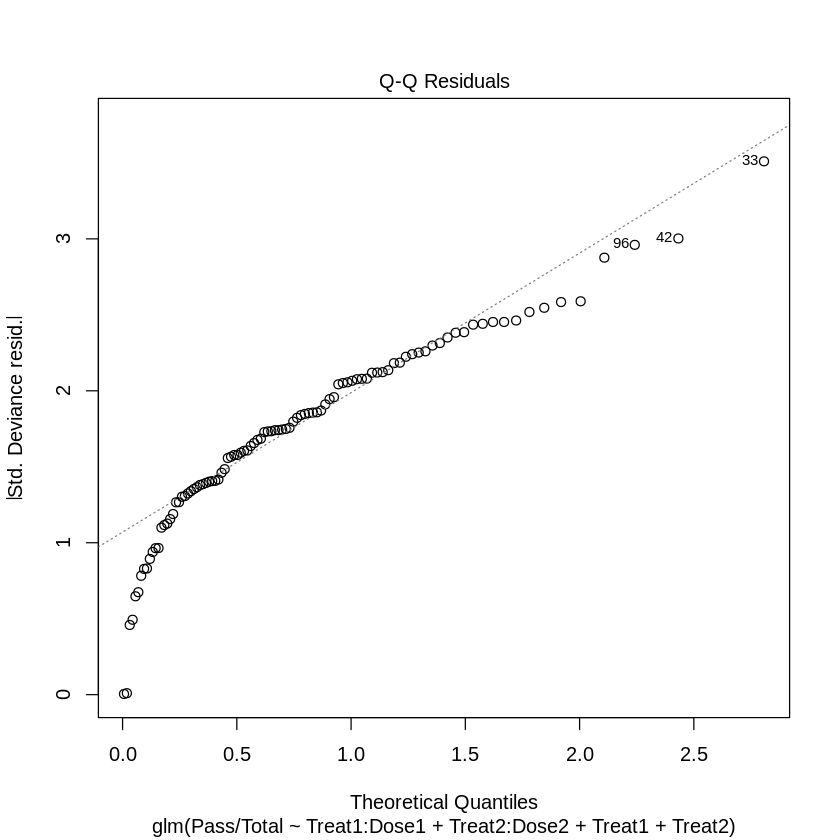
\includegraphics[width = \textwidth]{QQplot.png}
Here we can see that the tails are slightly heavy but the center
aligns very well with the theoretical distribution.

\subsubsection{Residual vs Fitted value}
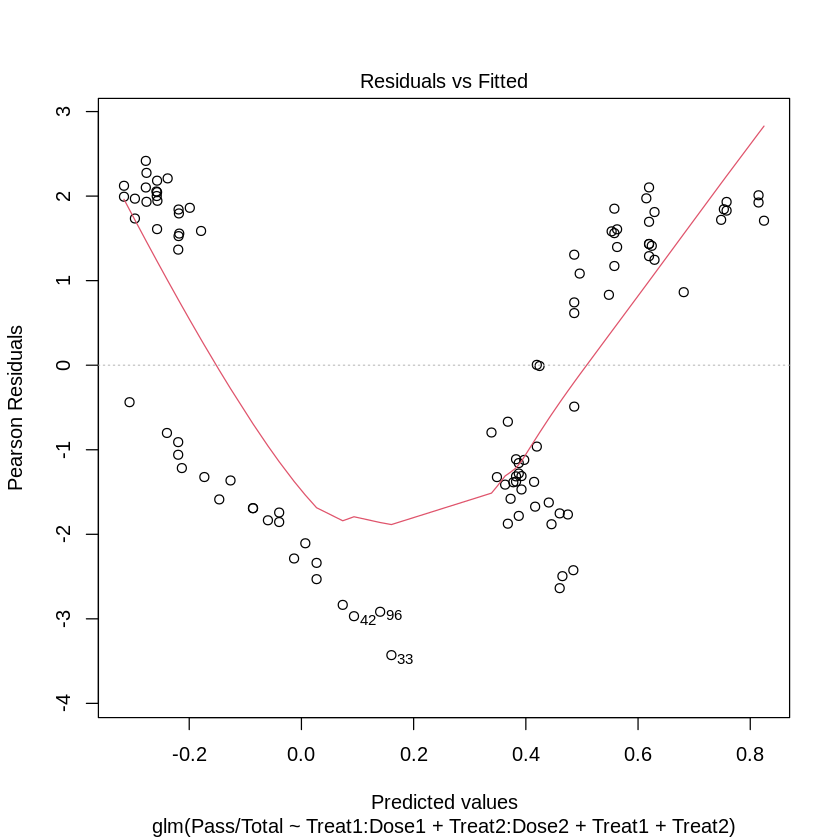
\includegraphics[width=\textwidth]{resvsfit.png}
This plot should be a flat line at 0 with points distributed around
the line but as we can see it is far from it.
\\
\\
For more details about the parameters of each model please check attached
R file.

\end{document}
